\section{Parameters}
In the experiments, a base network injection rate of 0.2 is assumed\footnote{The actual injection rate can be higher once \glspl{arq} come into play
and retransmissions are required.}
\begin{itemize}
    \item Injection rate
        \begin{itemize}
            \item Value if 0.2 is realistic
            \item Possibility to generate pairs for fair comparison of UC/NC
        \end{itemize}
    \item Overhead von Verschlüsselung+Auth vs. nur Auth vs keins von beiden (sowohl Latenz als auch Chipfläche)
\end{itemize}

\section{Attacker Model}
\begin{itemize}
    \item Focuses on malicious modifications rather than DoS attacks
    \item Assumption: compromised routers → rely on NIs for security
    \item No protection against bandwidth depletion, but this is not the goal here
    \item Variable number of compromised routers (e.g. 8 for an 8x8 grid)
    \item Compromised routers randomly drop or modify packets (no intelligent modifications/drops)
    \item Reasoning for having only some compromised routers (in regard to the 3rd party NoC problem → why would they not make all routers the same?)
        → HT implies more logic in routers → more area and draws more power → might attract attention if all routers have this and overall NoC
        parameters diverge considerably from the expectations
\end{itemize}

\section{Environment}
% 50,000 cycles (why?)
% Warmup and cooldown times
% Injection rate of 0.2 into the network

\section{Determining The Hyperparameters}
\subsection{ARQ Timeouts}\label{subsec:arqtimeouts}
Receivers issue \glspl{arq} when the temporal gap between the arrival of flits belonging to the same transmission unit becomes too large, i.e. when a
timeout occurs. Its value is determined through experiments and measured in clock cycles.

\begin{figure}
    \centering
    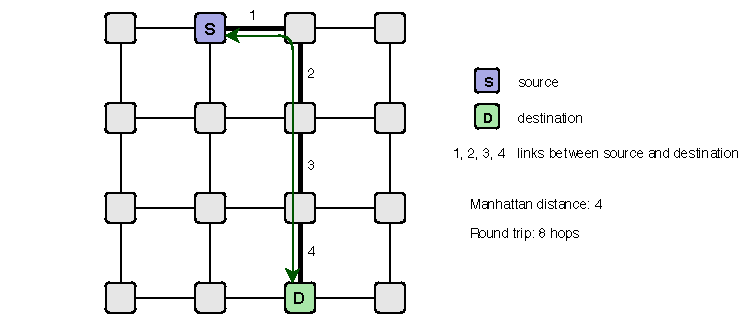
\includegraphics[width=0.9\textwidth]{arq-timeouts-calc}
    \caption[Example of ARQ timeout calculation]{Example for the calculation of \gls{arq} timeouts. With a Manhattan distance of 4 between source $S$ and
    destination $D$ and a given inter-arrival timeout $t_1$, the \gls{arq} timeout $t_2(S, D)$ is computed as $t_1 + 2 \cdot 4 = t_1 + 8$ cycles.}
    \label{fig:arqtimeoutscalc}
\end{figure}

In addition to the inter-arrival timeout, there is another, higher value that is used after an \gls{arq} was issued to await the answer, as explained
in Section \ref{subsec:arqretransmissions}. The \gls{arq} answer timeout depends on the inter-arrival timeout and the Manhattan distance between the
two affected communication partners. More precisely, if $t_1$ is the inter-arrival timeout, $t_2(S, D)$ is the \gls{arq} answer timeout for a
particular source $S$ and destination $D$, and $d$ is the Manhattan distance between the two nodes, then $t_2(S, D) = t_1 + 2 \cdot d$. Figure
\vref{fig:arqtimeoutscalc} illustrates this calculation.


As a starting point, a timeout of 8 cycles is used. It was identified as the optimal value in a previous diploma thesis about \gls{rlnc} for
\glspl{noc} \cite{yan15rlnc}. However, it may not be optimal for the scenarios investigated here since the protocol differs and a new simulator is
used with a different network interface structure.

\subsection{Number Of Crypto Units}

\section{Experiments}
\subsection{Average time of a flit/transmission unit in ArrivalManager until a verification result is there}
\subsection{Number of ARQs modified/dropped by routers}
\subsection{Routing strategies effects}
% Heatmap of router workload?

\iffalse
Experiment setup parameter tables:
- NC mode (UC, G2C3, G2C4)
- ...

ARQ Limit: 1, at most 2 because more ARQs allowed per transmission unit means larger retransmission buffers everywhere
\fi
